\documentclass{article}

\usepackage[a4paper, total={6in, 10in}]{geometry}
\usepackage{cite}
\usepackage{amsmath,amssymb,amsfonts}
\usepackage{algorithmic}
\usepackage{graphicx}
\usepackage{textcomp}
\usepackage{xcolor}
\usepackage{hyperref}

\usepackage{tikz}
\usetikzlibrary{shapes.geometric, arrows}

\tikzstyle{node} = [rectangle, rounded corners, minimum width=3cm, minimum height=1cm,text centered, draw=black]
\tikzstyle{arrow} = [thick,->,>=stealth]


\makeatletter

\renewcommand{\@seccntformat}[1]{}
\makeatother

\title{Effective Aircraft Boarding Strategies \\
\large{DAT530 Fall 2022 Project Proposal}}

\date{\today}

\author{Ali Seirafi (261854)\\ 
Rihab Al Zurkani (267102)\\ 
Stephan Frederik Werner Brandasu (245619)}

\begin{document}
\maketitle
\section{Project Description}
Boarding a plane often feels like a slow process which could be done better.
But is that true? and what is the best way for people to board a plane then?

For this project we want to model a few different methods of how passengers board
an aircraft and compare how long each method takes. This is an interesting
process to model and try to optimize because as they say 
'time is money' and neither the passengers nor the airline wants
to waste unnecessary time boarding the plane. 


\section{The Model}
The model it self will be the economy class layout of a single story wide-body aircraft. 
It doesn't matter which one we choose so here we've arbitrarily chosen the seat map of a
Boeing 787-10 from KLM which can be seen in figure \ref{fig:787seatmap}.

\begin{figure}[h]
    \centering
    \includegraphics[width=\textwidth]{KLM_Boeing_787-10.png}
    \caption{"Boeing 787-10 (781) KLM Seat Map", by SeatGuru \url{https://www.seatguru.com/airlines/KLM/KLM_Boeing_787-10.php}}
    \label{fig:787seatmap}
\end{figure}

We will only consider the economy class of the plane (marked in red) because
airlines usually allow higher paying passengers to board first as 
it is considered a perk of the ticket. 

In the economy class there are 3 rows of 3 seats each going to the back of the plane with 
2 isles on each side of the middle row. The problem that needs 
tackling is that when somebody wants to get to their seat they stop, 
stow their luggage and shuffle into their seat. But there is likely
somebody queueing behind them who has to stand and wait for the person 
in front to finish before they can proceed to their own seat. 

So then a logical way of filling up the plane would be a normal back to front
approach, but you can't make people queue row for row 
to enter the plane, this would take far too much organization. So instead 
the passengers get divided into a number subgroups, going back to front to try to minimize
the waiting time where somebody is blocking you because they're stowing
their luggage, but it will still partially exist. 

Well that seems to make sense on the surface but how many groups 
should we divide passengers into and how much better is it than just 
doing a free for all approach?

Another issue besides just waiting for people to stow their luggage is the 
seat shuffle, where somebody who is sitting near the isle gets to their seat first 
and then has to get up when the people not in the aisle get to their seat. How much
does this matter and could we combat it?

The approach against that could be to group the passengers
by column instead of by row. So let the people sitting by the windows board first 
and then work our way in from there. This would eliminate the blockage from
the seat shuffle but would still keep the issue from people 
entering the plane in the wrong order. 

So at that point the logical conclusion would be to try to combine
the row grouping with the column grouping in some way to try to avoid the 
isle blocking and the seat shuffle at the same time, but again we can't
have too many boarding groups so it needs to be simulated if this is even
worth it.

These are some examples of approaches to boarding a plane that can be tested and 
compared to each other to try to find the best approach to boarding a plane. 

\section{The Process}

\begin{center}
\begin{figure}[h]
    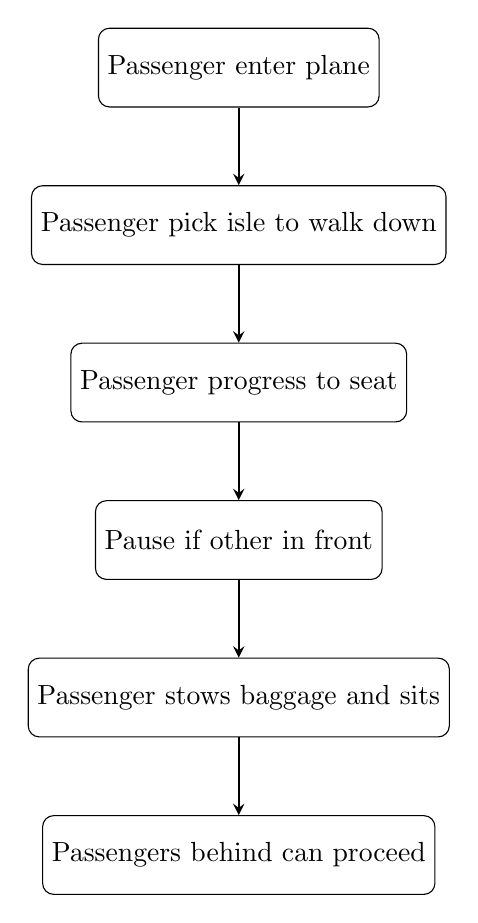
\begin{tikzpicture}[node distance=2cm]
        \node (start) [node] {Passenger enter plane};
        \node (two) [node, below of=start] {Passenger pick isle to walk down};
        \draw [arrow] (start) -- (two);
        \node (three) [node,  below of=two] {Passenger progress to seat};
        \draw [arrow] (two) -- (three);
        \node (four) [node,  below of=three] {Pause if other in front};
        \draw [arrow] (three) -- (four);
        \node (five) [node,  below of=four] {Passenger stows baggage and sits};
        \draw [arrow] (four) -- (five);
        \node (six) [node,  below of=five] {Passengers behind can proceed};
        \draw [arrow] (five) -- (six);
    \end{tikzpicture}
    \caption{simplified model of passenger decision process}
    \label{fig:simp_model}
\end{figure}
\end{center}

In figure \ref{fig:simp_model} we show a simplified model of what the passenger has to account
for when entering the plane. 


\section{Summary}
So in summary we want to compare how long it takes to:
\begin{enumerate}
    \item Board everyone free for all
    \item Board everyone front to back
    \item Board everyone column by column
    \item A combination of 2 and 3
\end{enumerate}


\end{document}